\documentclass[border=10pt]{standalone}
\usepackage{tikz}\usepackage{amsmath}\usetikzlibrary{arrows.meta}
\begin{document}
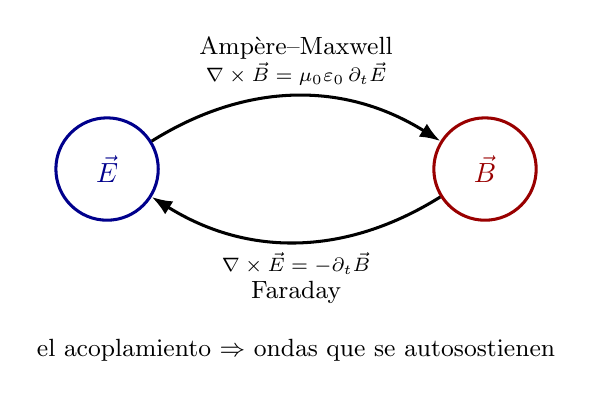
\begin{tikzpicture}[line width=0.9pt,>={Latex[length=2.6mm]}]
  \node[draw,circle,line width=1.1pt,minimum size=1.3cm,blue!55!black] (E) at (-2.4,0){$\vec E$};
  \node[draw,circle,line width=1.1pt,minimum size=1.3cm,red!60!black] (B) at (2.4,0){$\vec B$};
  \draw[->,line width=1.1pt] (E) to[bend left=32] node[above,align=center]{\small Ampère–Maxwell\\[-2pt]\scriptsize $\nabla\times\vec B=\mu_0\varepsilon_0\,\partial_t\vec E$} (B);
  \draw[->,line width=1.1pt] (B) to[bend left=32] node[below,align=center]{\scriptsize $\nabla\times\vec E=-\partial_t\vec B$\\[-2pt]\small Faraday} (E);
  \node at (0,-2.3){\small el acoplamiento $\Rightarrow$ ondas que se autosostienen};
\end{tikzpicture}
\end{document}
